\begin{frame}
    \frametitle{\problemtitle}
    \begin{description}
        \item<+->[Problem:] How many times do you need to move the joystick up or down to enter your initials?
        \item<+->[Observation:] Each letter position can be treated individually.
        \item<+->[Solution:] Sum, for all pairs of letters, the ``distance'' on the alphabet wheel:
    \end{description}

    \uncover<.->{
        \begin{columns}
            \hfill
            \column{0.25\textwidth}
            \begin{center}
                % Inspired by https://tex.stackexchange.com/a/103368
                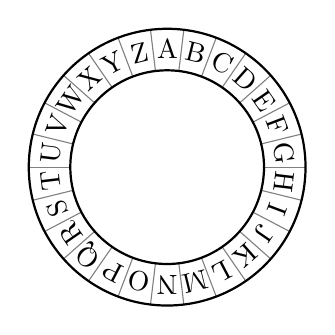
\begin{tikzpicture}
                    \pgfmathsetmacro{\alphsize}{26}

                    \pgfmathsetmacro{\angl}{360/\alphsize}
                    \pgfmathsetmacro{\d}{10}
                    \pgfmathsetmacro{\op}{98 + \angl/2 - 1.2}
                    \pgfmathsetmacro{\e}{\angl + \angl*\d}
                    \pgfmathsetmacro{\ep}{\op + \angl*\d}

                    \foreach \x in {0,\angl,...,360} {
                        \draw[gray] (\x:3.5em) -- (\x:5em);
                    }

                    \foreach \x [count=\xi] in {A,...,Z} {
                        \node[rotate=\angl - \angl*\xi] at (\op - \angl*\xi:4.25em) {\x};
                    }

                    \draw[thick] (0em,0em) circle(5em);
                    \draw[thick] (0em,0em) circle(3.5em);
                \end{tikzpicture}
            \end{center}

            \column{0.45\textwidth}
            \[ \sum_{(a,b)} \min(a - b \mod 26, b - a \mod 26) \]
        \end{columns}
    }
    \solvestats
\end{frame}
